\documentclass[border=0bp]{standalone}
\usepackage{newtxtext,newtxmath}
\usepackage{tikz}
\usetikzlibrary{arrows.meta,calc}
\definecolor{teal}{HTML}{167C80}
\definecolor{orange}{HTML}{D55E00}
\definecolor{blue}{HTML}{0072B2}
\definecolor{gray}{HTML}{59636A}
\definecolor{ink}{HTML}{23343B}
\definecolor{hard}{HTML}{C43C39}
\DeclareMathSizes{7.5}{7.5}{7.2}{7.2}
\DeclareMathSizes{8}{8}{7.2}{7.2}
\DeclareMathSizes{8.8}{8.8}{7.2}{7.2}
\DeclareMathSizes{9}{9}{7.2}{7.2}
\DeclareMathSizes{10}{10}{7.2}{7.2}
\newcommand{\bodyfont}{\fontsize{7.5}{8.5}\selectfont}
\newcommand{\titlefont}{\fontsize{8.8}{9.6}\selectfont\bfseries}
\newcommand{\mathfont}{\fontsize{9}{10}\selectfont}
\tikzset{
  every node/.style={font=\bodyfont,text=ink,inner sep=0pt,outer sep=0pt},
  module/.style={rounded corners=3bp,line width=.6bp},
  flow/.style={line width=.8bp,-{Stealth[length=3.5bp,width=3bp]}},
  edge/.style={line width=1.2bp,shorten <=3.3bp,shorten >=3.3bp,-{Stealth[length=3bp,width=2.7bp]}},
  title/.style={font=\titlefont},
  formula/.style={font=\mathfont},
  label/.style={fill=white,inner sep=1.5bp}
}
\begin{document}
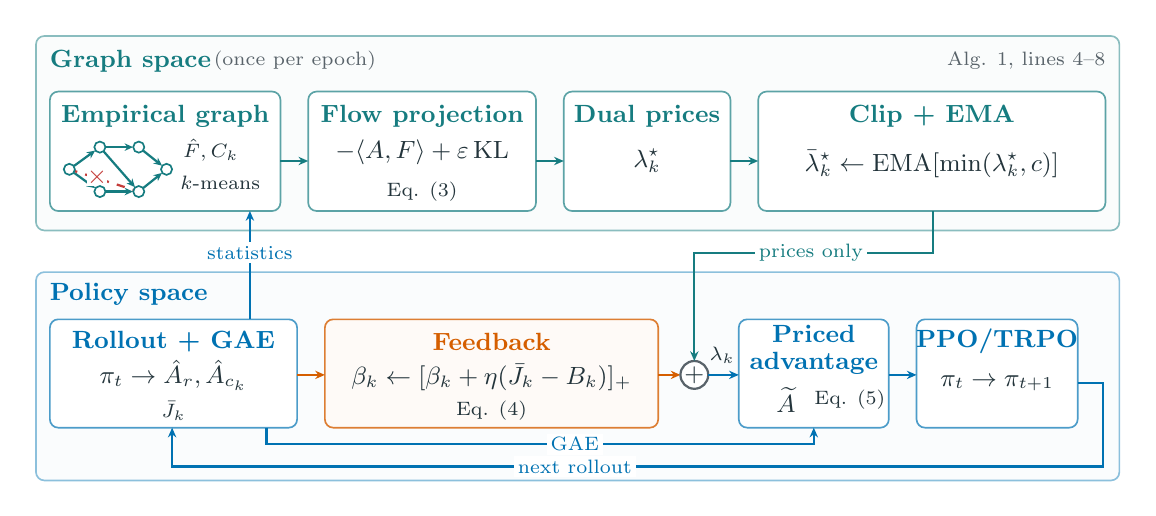
\begin{tikzpicture}[x=1bp,y=-1bp]

\path[use as bounding box] (0,0) rectangle (396,165.6);
% Two bands with one internal module level. Left-to-right within each band.
\draw[module,draw=teal!50,fill=teal!2] (3,3) rectangle (393,73);
\draw[module,draw=blue!45,fill=blue!2] (3,88) rectangle (393,163);
\node[title,text=teal,anchor=west] at (8,12) {Graph space};
\node[anchor=west,text=gray] at (67,12) {(once per epoch)};
\node[anchor=east,text=gray] at (388,12) {Alg. 1, lines 4--8};
\node[title,text=blue,anchor=west] at (8,96) {Policy space};

\draw[module,draw=teal!70,fill=white] (8,23) rectangle (91,66);
\draw[module,draw=teal!70,fill=white] (101,23) rectangle (183,66);
\draw[module,draw=teal!70,fill=white] (193,23) rectangle (253,66);
\draw[module,draw=teal!70,fill=white] (263,23) rectangle (388,66);
\node[title,text=teal] at (49.5,32) {Empirical graph};
\node[title,text=teal] at (142,32) {Flow projection};
\node[title,text=teal] at (223,32) {Dual prices};
\node[title,text=teal] at (325.5,32) {Clip + EMA};

\foreach \name/\x/\y in {g0/15/51,g1/26/43,g2/40/43,g3/26/59,g4/40/59,g5/50/51}
 \coordinate (\name) at (\x,\y);
\foreach \a/\b in {g0/g1,g1/g2,g2/g5,g0/g3,g3/g4,g4/g5,g1/g4}
 \draw[edge,teal,line width=.8bp,shorten <=2.1bp,shorten >=2.1bp] (\a) -- (\b);
\draw[hard,dashed,line width=.8bp] (g0) -- (g4);
\node[text=hard,fill=white,font=\fontsize{9}{9}\selectfont] at (25,54) {$\times$};
\foreach \name in {g0,g1,g2,g3,g4,g5}
 \filldraw[draw=teal,fill=white,line width=.6bp] (\name) circle (2bp);
\node[anchor=west] at (56,44) {$\hat F,C_k$};
\node[anchor=west] at (55,56) {$k$-means};
\node[formula] at (142,45) {$-\langle A,F\rangle+\varepsilon\,\mathrm{KL}$};
\node at (142,59) {Eq. (3)};
\node[formula] at (223,48) {$\lambda_k^\star$};
\node[formula] at (325.5,49) {$\bar\lambda_k^\star\leftarrow\mathrm{EMA}[\min(\lambda_k^\star,c)]$};
\draw[flow,teal] (91,48) -- (101,48);
\draw[flow,teal] (183,48) -- (193,48);
\draw[flow,teal] (253,48) -- (263,48);

\draw[module,draw=blue!70,fill=white] (8,105) rectangle (97,144);
\draw[module,draw=orange!80,fill=orange!3] (107,105) rectangle (227,144);
\draw[module,draw=blue!70,fill=white] (256,105) rectangle (310,144);
\draw[module,draw=blue!70,fill=white] (320,105) rectangle (378,144);
\node[title,text=blue] at (52.5,113) {Rollout + GAE};
\node[formula] at (52.5,125) {$\pi_t\to\hat A_r,\hat A_{c_k}$};
\node at (52.5,138) {$\bar J_k$};
\node[title,text=orange] at (167,113) {Feedback};
\node[formula] at (167,126) {$\beta_k\leftarrow[\beta_k+\eta(\bar J_k-B_k)]_+$};
\node at (167,138) {Eq. (4)};
\node[title,text=blue,align=center] at (283,116) {Priced\\advantage};
\node[formula] at (273,134) {$\widetilde A$};
\node at (296,134) {Eq. (5)};
\node[title,text=blue] at (349,113) {PPO/TRPO};
\node[formula] at (349,128) {$\pi_t\to\pi_{t+1}$};

% Input paths have distinct meanings; GAE bypasses graph and feedback.
\draw[flow,orange] (97,125) -- (107,125);
\draw[flow,orange] (227,125) -- (235,125);
\draw[line width=.8bp,gray,fill=white] (240,125) circle (5bp);
\node[formula] at (240,125) {$+$};
\draw[flow,blue] (245,125) -- (256,125);
\node[anchor=south] at (250,121) {$\lambda_k$};
\draw[flow,blue] (310,125) -- (320,125);
\draw[flow,teal] (326,66) -- (326,81) -- (240,81) -- (240,120);
\node[label,text=teal] at (282,81) {prices only};
\draw[flow,blue] (80,105) -- (80,66);
\node[label,text=blue] at (80,81) {statistics};
\draw[flow,blue] (86,144) -- (86,150) -- (283,150) -- (283,144);
\node[label,text=blue] at (197,150) {GAE};
\draw[flow,blue] (378,128) -- (387,128) -- (387,158) -- (52,158) -- (52,144);
\node[label,text=blue] at (197,158) {next rollout};
\end{tikzpicture}
\end{document}
